\documentclass[11pt]{exam}
\usepackage{../commonheader}
\usepackage{graphicx}

\title{Matrices \& Gaussian Elimination}
\date{Week 1, Session 2}

\begin{document}
\maketitle

\section{Matrices}
    
    \vspace{20px}
    \subsection{Augmented Matrices}
        \begin{questions}
            \item Convert the following linear systems into augmented matrices:
            \begin{enumerate}
                \item $\begin{cases}
                    2x + 2y = 1 \\
                    x = 4
                    \end{cases}$
                \item $\begin{cases}
                    4x + 3y - 2z = 1 \\
                    6x = 3y + 4z + 7 \\
                    8z + 12x + 14y = 13 \\
                    y = 4
                    \end{cases}$
            \end{enumerate}
            
            \item Suppose you have a \textbf{two-variable} linear system with \textbf{three} equations. How many rows and columns will
            the \textit{augmented matrix} for the system have?

            \item Suppose you construct an augmented matrix using a linear system, then you double every entry of the matrix. What effect will 
            the doubling have on the solutions of the system?
        \end{questions}

        \vspace{20px}
        \subsection{Elementary Row Operations}
        \begin{questions}
            \item Use elementary row operations on the following matrices to cancel out as many entries as possible in the last row:
            \begin{enumerate}
                \item $\begin{bmatrix}
                    1 & 2 & 4 \\
                    2 & 3 & 4 \\
                    4 & 10 & 7
                \end{bmatrix}$
                \item $\begin{bmatrix}
                    2 & 5 & 3 \\
                    0 & 1 & 4 \\
                    2 & 6 & 7
                \end{bmatrix}$
            \end{enumerate}
        \end{questions}

\pagebreak
\section{Row-Echelon and Reduced Row-Echelon Forms}

    \vspace{20px}
    \subsection{Leading Entries and Pivots}
        To understand row-echelon form, you first must have a grasp of the concept of a \textit{leading entry}.
        In short, a leading entry is the leftmost nonzero entry in a given row. For example, the boxed entries in the following matrix:
        $$\begin{bmatrix}
            \boxed{1} & 1 & 1 & 1 & 1 \\
            0 & 0 & \boxed{2} & 0 & 1 \\
            0 & \boxed{3} & 1 & 1 & 2 \\
            0 & 0 & 0 & 0 & \boxed{4}
        \end{bmatrix}$$
        Another name for leading entries is \textit{pivot positions}. Columns which have a pivot position are known as \textit{pivot columns}.
        In the example above, all columns but the fourth are pivot columns.
        \begin{questions}
            \item Identify the pivot positions and columns in the following matrix:
            $$\begin{amatrix}{6}
                1 & 0 & 0 & 2 & 3 & 12 & 0 \\
                0 & 0 & 2 & 3 & 2 & 2 & 1 \\
                0 & 0 & 0 & 0 & 4 & 3 & 6 \\
                0 & 0 & 0 & 0 & 0 & 0 & 5
            \end{amatrix}$$
        \end{questions}
    
    \vspace{20px}
    \subsection{Row-Echelon Form}
        Recall the definition for row-echelon form:
        An augmented matrix is in \textbf{row-echelon form} if:
        \begin{enumerate}
            \item All nonzero rows are above any rows of zeros.
            \item Each leading entry of a row is in a column to the right of the leading entries of any row above it.
            \item Each leading entry of a row is equal to 1.
        \end{enumerate}

        That's pretty wordy, so maybe this wording will make a bit more sense:
        \begin{enumerate}
            \item Any zeroed-out rows should be stacked at the very bottom of the matrix.
            \item As you descend downwards from the top row, any leading entries in new rows should be right of all previous ones.
            \item All leading entries are 1.
        \end{enumerate}
        Let's look at some examples!

        \pagebreak
        \begin{questions}
            \item Consider the above rules, and classify whether the following matrices are in row-echelon form or not.
            Explain which rule each violates (if any):
            \begin{enumerate}
                \item $\begin{amatrix}{3}
                    0 & 0 & 0 & 0 \\
                    1 & 2 & 3 & 3 \\
                    0 & 1 & 0 & 2 \\
                    0 & 0 & 0 & 1 \\
                    0 & 0 & 0 & 0
                \end{amatrix}$
                \item $\begin{amatrix}{5}
                    1 & 0 & 6 & 5 & 8 & 2 \\
                    0 & 0 & 1 & 2 & 7 & 3 \\
                    0 & 0 & 0 & 0 & 1 & 1 \\
                    0 & 0 & 0 & 0 & 0 & 0
                \end{amatrix}$
                \item $\begin{amatrix}{2}
                    1 & 2 & 3 \\
                    2 & 4 & -6 \\
                    4 & 0 & 7
                \end{amatrix}$
                \item $\begin{amatrix}{3}
                    1 & 3 & 5 & 4 \\
                    0 & 1 & 0 & 7 \\
                    0 & 0 & 1 & 0 \\
                    0 & 0 & 0 & 1 \\
                    0 & 0 & 0 & 0
                \end{amatrix}$
                \item $\begin{amatrix}{3}
                    1 & 0 & 6 & 0 \\
                    0 & 1 & 4 & 0 \\
                    0 & 0 & 1 & 0 \\
                    0 & 0 & 0 & 0
                \end{amatrix}$
                \item $\begin{amatrix}{3}
                    0 & 2 & 3 & 3 \\
                    1 & 5 & 0 & 2 \\
                    7 & 5 & 0 & 1 \\
                    0 & 0 & 1 & 0
                \end{amatrix}$
            \end{enumerate}
        \end{questions}

    \pagebreak
    \subsection{Reduced Row-Echelon Form}
        The rules for reduced row-echelon form are the same as row-echelon, with one addition:
        \begin{enumerate}
            \item All entries in a column above and below a leading entry are zero.
        \end{enumerate}
        For example, the following matrix is in row-echelon form, but not in reduced row-echelon form (commonly written as RREF).
        In order to get it to RREF, the boxed entries would need to be cancelled so that there are no nonzero entries above the leading entries.
        $$\begin{bmatrix}
            1 & \boxed{1} & \boxed{1} \\
            0 & 1 & \boxed{1} \\
            0 & 0 & 1
        \end{bmatrix}$$

        \begin{questions}
            \item Determine whether the following matrices are in RREF, row-echelon form, or neither.
            \begin{enumerate}
                \item $\begin{amatrix}{5}
                    1 & 0 & 0 & 5 & 0 & 0 \\
                    0 & 0 & 1 & 2 & 0 & 0 \\
                    0 & 0 & 0 & 0 & 1 & 1 \\
                    0 & 0 & 0 & 0 & 0 & 0
                \end{amatrix}$
                \item $\begin{amatrix}{3}
                    1 & 0 & 0 & 4 \\
                    0 & 1 & 0 & 3 \\
                    0 & 0 & 1 & 2
                \end{amatrix}$
                \item $\begin{bmatrix}
                    1 & 0 & 2 & 3 & 4 \\
                    0 & 1 & 5 & 6 & 7 \\
                    0 & 0 & 0 & 1 & 8 \\
                    0 & 0 & 0 & 0 & 1
                \end{bmatrix}$
                \item $\begin{bmatrix}
                    1 & 0 & 3 & 6 \\
                    0 & 1 & 4 & 6 \\
                    0 & 1 & 0 & 0
                \end{bmatrix}$
            \end{enumerate}

            \item Use row operations to convert the following matrices to RREF:
            \begin{enumerate}
                \item $\begin{bmatrix}
                    -1 & 1 \\
                    -1 & 0 \\
                    0 & -1 \\
                    -1 & -2
                \end{bmatrix}$
                \item $\begin{bmatrix}
                    0 & 1 & 3 \\
                    -1 & -3 & 3 \\
                    1 & -3 & 0
                \end{bmatrix}$
                \item $\begin{bmatrix}
                    -1 & 1 \\
                    -1 & 2 \\
                    -3 & 2
                \end{bmatrix}$
            \end{enumerate}
        \end{questions}

\pagebreak
\section{Solving Linear Systems in Matrix Form}

    \vspace{20px}
    \subsection{Solving Systems Using Gauss-Jordan Elimination}
    Gauss-Jordan elimination is the process of performing row operations on the augmented matrix of a linear system to find its solution(s).
    \begin{questions}
        \item Use Gauss-Jordan elimination to solve the following linear systems:
        \begin{enumerate}
            \item $\begin{amatrix}{2}
            1 & 1 & 0 \\
            2 & 6 & 4
            \end{amatrix}$
            \item $\begin{bmatrix}
                1 & 2 & 0 \\
                4 & 8 & 4
            \end{bmatrix}$
        \end{enumerate}
    \end{questions}

    \vspace{20px}
    \subsection{Systems with Infinite Sets of Solutions}
        Sometimes, a linear system will have an infinite set of solutions instead of one specific solution. What does this look like when using
        Gauss-Jordan elimination, and how can we "solve" for an infinite set of solutions? Let's consider an example, already reduced to RREF:
        $$\begin{amatrix}{3}
            1 & 0 & -5 & -3 \\
            0 & 1 & -10 & 0 \\
            0 & 0 & 0 & 0
        \end{amatrix}$$
        This corresponds to the set of equations $\begin{cases}
            x - 5z = 3 \\
            y - 10z = 0
        \end{cases}$
        or $\begin{cases}
            x = 3 + 5z \\
            y = 10z
        \end{cases}$

        Note that you could choose any value of $z$, and the set of values $(x,y,z) = (3 + 5z, 10z, z)$ will be a solution! So how can we rigidly define
        this behavior as our "solution"?

        We can allow $z$ take on the value of a \textit{parameter} $t$, and then define our solution vector as:
        $$\begin{bmatrix} x \\ y \\ z \end{bmatrix} = \begin{bmatrix} 3 + 5t \\ 10t \\ t \end{bmatrix}$$
        
        We can take this a step further and split the vector up by like terms, and obtain:
        $$\begin{bmatrix} x \\ y \\ z \end{bmatrix} = \begin{bmatrix} 3 \\ 0 \\ 0 \end{bmatrix} + t\begin{bmatrix} 5 \\ 10 \\ 1 \end{bmatrix}$$

        Let's try to build some intuition on this. Since we have two equations in three variables, we could represent the system as two planes in 3D space.
        These planes can either not intersect at all (they're parallel), intersect along a line in 3D space (if they "cross" each other),
        or intersect along a surface in 3D space (if they're the same plane).

        \begin{center}
            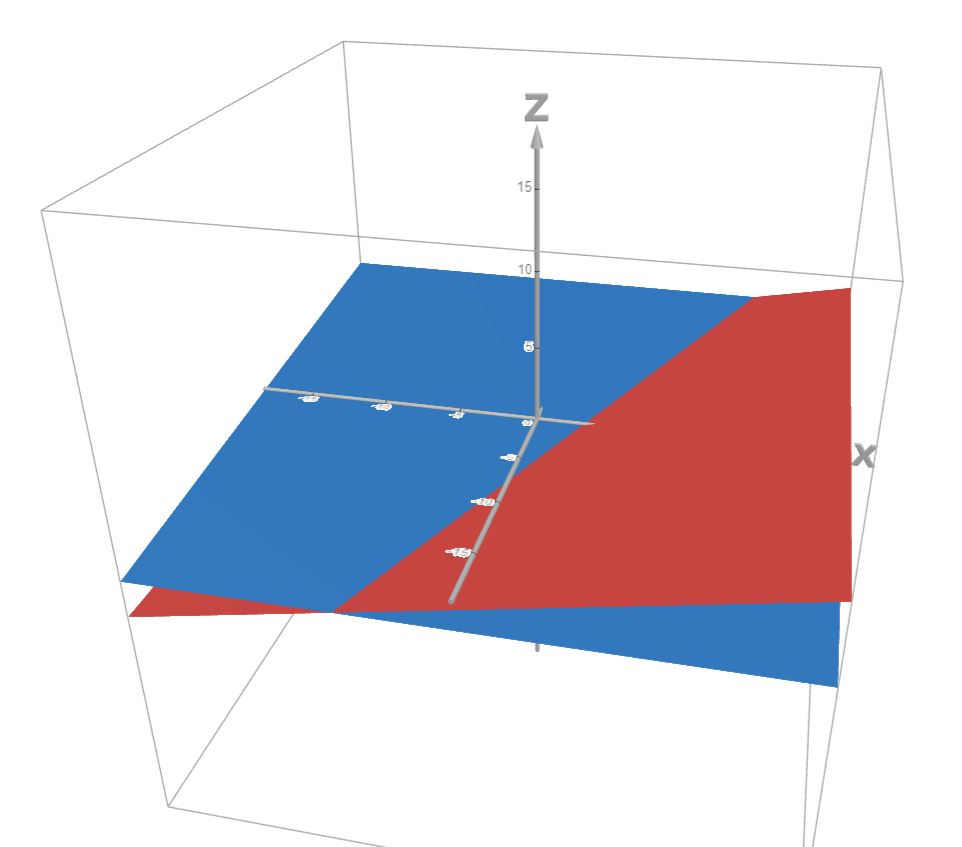
\includegraphics[width=0.5\textwidth]{planes.JPG}
        \end{center}

        Graphically, the planes in this system intersect along a line! It turns out that our solution set \text{it} is just be a representation of that line.
        For those of you who have taken Calculus 3, our solution should be familiar as the equation of a vector-valued function.

        In the image below, the dots correspond with $t = -1, t = 0$, and $t = 1$ from left to right.

        \begin{center}
            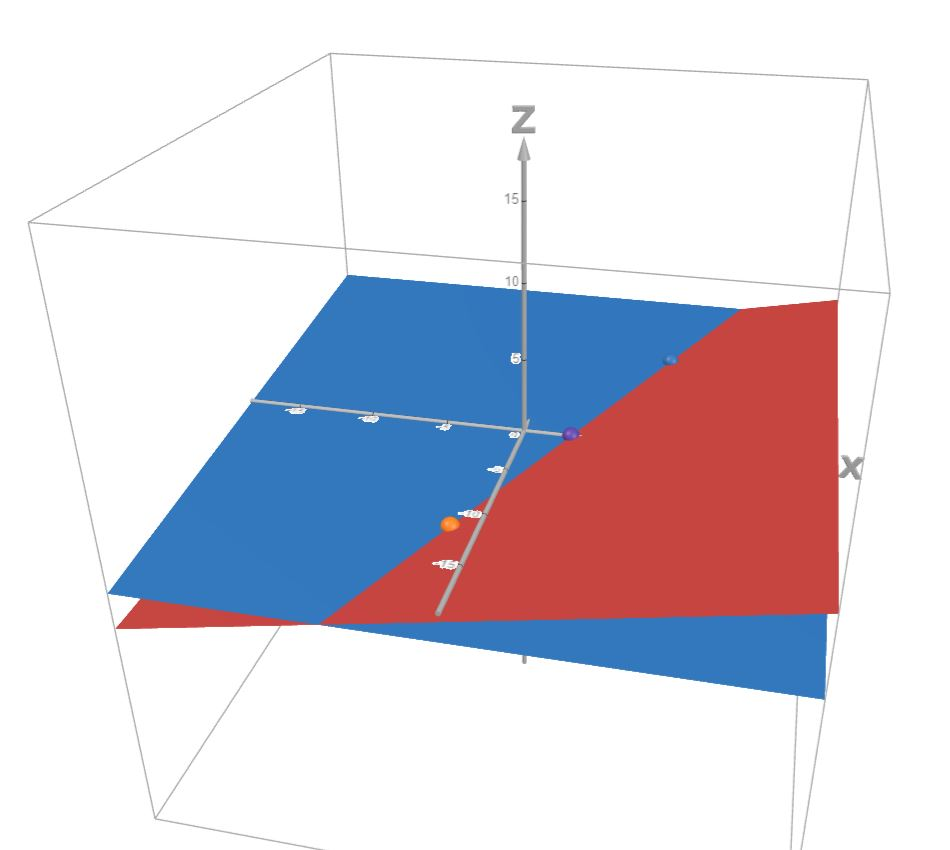
\includegraphics[width=0.5\textwidth]{planes_with_points.JPG}
        \end{center}

        \begin{questions}
            \item How do you think the solution set would differ if we had a similar system where the planes intersected along a surface instead of a line?
            \pagebreak
            \item Find the infinite set of solutions to the system represented by the following augmented matrix:
            $$\begin{amatrix}{4}
                1 & 2 & -1 & 1 & 3 \\
                1 & 1 & -1 & 1 & 1 \\
                1 & 3 & -1 & 1 & 5
            \end{amatrix}$$
        \end{questions}

    \vspace{20px}
    \subsection{Pivot Columns and Infinite Sets of Solutions}
    It turns out that each non-pivot column in the RREF of an augmented matrix corresponds with one additional parameter being used in the infinite
    set of solutions of the associated linear system.

    Consider the following system:
    $$\begin{amatrix}{4}
        1 & 0 & 0 & 0 & 5 \\
        0 & 1 & 2 & 0 & -3
    \end{amatrix}$$
    We could rewrite the system in equation form using two parameters, $s$ and $t$:
    $$\begin{cases}
        x = 5 \\
        y = -2z - 3 \\
        z = s \\
        w = t
    \end{cases}$$
    Using the parameters, we can write the solution as:
    $$\begin{bmatrix} x \\ y \\ z \\ w \end{bmatrix} = \begin{bmatrix} 5 \\ -2s - 3 \\ s \\ t \end{bmatrix}
    = \begin{bmatrix} 5 \\ -3 \\ 0 \\ 0 \end{bmatrix}
    + s\begin{bmatrix} 0 \\ -2 \\ 1 \\ 0 \end{bmatrix}
    + t\begin{bmatrix} 0 \\ 0 \\ 0 \\ 1 \end{bmatrix}$$

    Recall that the original matrix had two non-pivot columns; this is why we had two parameters in the solution! When we have a variable
    that is assigned to a parameter, we refer to that variable as a \textit{free variable}. In the above example, $z$ and $w$ are free variables.

    \begin{questions}
        \item How many parameters would the following augmented matrix have in its solution set?
        $$\begin{amatrix}{3}
            1 & 0 & 2 & 4 \\
            0 & 1 & 4 & 0
        \end{amatrix}$$ 
    \end{questions}

\pagebreak
\section{Closing}
    Great job today! Let's finish up with a few quick recap questions to close it out.
    \begin{questions}
        \item What is a pivot column?
        \item True or false? All leading entries must be 1 in row-echelon form.
        \item True or false? All entries above a pivot position must be 0 in RREF.
        \item \textbf{Challenge question: } A two-variable system has \textbf{two} free variables. What is the set of solutions of the system? 
    \end{questions}
    

\end{document}